The Raspberry Pi carries out three main duties to ensure everything works correctly. These include creating a wireless connection, streaming images from the camera to the phone and transmitting the data received from the phone to the microcontroller.\\

 These are all placed into the \textit{/etc/rc.local} file so the system initializes them automatically each time the robot is turned on, with no need for human interaction.

\subsection{Wireless Communications}% WiFi Acces Point

The chosen means of communication between human and humanoid was wifi. This is so because it is a widely established technology, with great compatibility and in a great number of cases is already installed in the homes of users. It also has a greater speed and range than other technologies, like bluetooth, which are an asset in the case of streaming images.\\

Three methods were considered: connection to an existing wifi network, creation of an Ad-Hoc connection and establishment of a wifi Access Point.

\subsubsection{Existing network:}

The most straightforward solution is to simply connect the robot to the user's existing wifi network. This enables the user to control it from anywhere in the world, expanding its uses. However, some configuration is required, namely selecting the desired network and introducing the password, which complicates the setup by having to add a keyboard and a display.\\

This method would thus be suitable for experienced users and developpers, but not necessarily for the average seniors it is intended to help.

\subsubsection{Ad-Hoc connection:}

The next solution implemented was an Ad-Hoc connection between the Raspberry Pi and the Android phone.\\

This configuration aimed to solve the problem of usability, since the phone would automatically connect to the network, hence eradicating the problem of setting up the communication.  This also had the advantage of creating an independent network, and thus being able to operate in remote areas. \\

In order to create implement this two files need to be set up. Firstly, the computer must be given the specific details of the new network to be created. Here, the contents of Listing \ref{ad-hoc} must be included into the file \textit{/etc/network/interfaces} . \\

	\begin{minipage}{\linewidth}%to ensure it stays in the same page
	\begin{lstlisting}[label=ad-hoc,caption=Ad-Hoc Configuration {[} /etc/network/interfaces {]} ,language=python ]
  auto lo
  iface lo inet loopback
  iface eth0 inet dhcp
 
  auto wlan0
  iface wlan0 inet static
    address 192.168.1.1
    netmask 255.255.255.0
    wireless-channel 1
    wireless-essid RPiAdHocNetwork
    wireless-mode ad-hoc
	\end{lstlisting}
	\end{minipage}

\bigskip
With this configuration the Raspberry will assign itself the IP address 192.168.1.1, but the client computer will be left without an IP assigned and so will be unable to connect to the former. 

To provide an IP to the client the package \textit{DHCP Server} must be installed by typing \textit{sudo apt-get install dhcp3-server} into a terminal. \\

Listing \ref{dhcp-server-adhoc} must then be included in file \textit{/etc/dhcp/dhcpd.conf} \\

	\begin{minipage}{\linewidth}%to ensure it stays in the same page
	\begin{lstlisting}[label=dhcp-server-adhoc,caption=DHCP Server Configuration {[} /etc/dhcp/dhcpd.conf {]} ,language=python ]
  ddns-update-style interim;
  default-lease-time 600;
  max-lease-time 7200;
  authoritative;
  log-facility local7;
  subnet 192.168.1.0 netmask 255.255.255.0 {
		  range 192.168.1.5 192.168.1.150;
  }
	\end{lstlisting}
	\end{minipage}

\bigskip	
After rebooting the Raspberry Pi, the Ad-Hoc network is created and ready to use. However, while it is compatible with a large range of devices like computers and iOs devices, non-rooted Android devices are not able to connect to the network, which invalidates this procedure as it is not suited for the general public.


\subsubsection{Wifi Access Point:}

The last option for connecting the phone to the robot is to create a wifi Access Point (AP). This method involves a more complex setup than the previous, but while maintaining the same benefits, both allows Android devices to connect and supports speeds of up to 54 Mbps in 802.11g, while the former was limited to 11 Mbps in 802.11b.\\

In order to create the AP the  \textit{Hostapd} and  \textit{Isc-dhcp-server} packages have to be installed: \textit{sudo apt-get install hostapd isc-dhcp-server}.\\

Once the needed packages have been installed the Dynamic Host Configuration Protocol (DHCP) server must be configured in order to assign IP addresses to clients. The contents of \textit{/etc/dhcp/dhcpd.conf} must be replaced with those in Listing \ref{dhcp-server-ap}. \\

	\begin{minipage}{\linewidth}%to ensure it stays in the same page
	\begin{lstlisting}[label=dhcp-server-ap,caption=DHCP Server Configuration {[} /etc/dhcp/dhcpd.conf {]} ,language=python ]
  # Sample configuration file for ISC dhcpd for Debian
  # Attention: If /etc/ltsp/dhcpd.conf exists, that will be used as
  # configuration file instead of this file.

  # The ddns-updates-style parameter controls whether or not the server
  # will attempt to do a DNS update when a lease is confirmed. We default 
  # to the behavior of the version 2 packages ('none', since DHCP v2 
  # didn't have support for DDNS.)
  ddns-update-style none;

  default-lease-time 600;
  max-lease-time 7200;

  # If this DHCP server is the official DHCP server for the local
  # network, the authoritative directive should be uncommented.
  authoritative;

  # Use this to send dhcp log messages to a different log file 
  log-facility local7;

  subnet 192.168.42.0 netmask 255.255.255.0 {
  range 192.168.42.10 192.168.42.50;
  option broadcast-address 192.168.42.255;
  option routers 192.168.42.1;
  default-lease-time 600;
  max-lease-time 7200;
  option domain-name "local";
  option domain-name-servers 8.8.8.8, 8.8.4.4;
  }
	\end{lstlisting}
	\end{minipage}

\bigskip
The next step is to establish the interface on which DHCP Server should assign IP addresses. This is done by copying the contents of Listing \ref{dhcp-server-defaults} to the file \textit{/etc/default/isc-dhcp-server}.\\

	\begin{minipage}{\linewidth}%to ensure it stays in the same page
	\begin{lstlisting}[label=dhcp-server-defaults,caption=DHCP Server Defaults {[} /etc/default/isc-dhcp-server {]} ,language=python ]
  # Defaults for dhcp initscript
  # sourced by /etc/init.d/dhcp
  # installed at /etc/default/isc-dhcp-server by the maintainer scripts

  #
  # This is a POSIX shell fragment
  #

  # On what interfaces should the DHCP server (dhcpd) serve requests?
  # Separate multiple interfaces with spaces, e.g. "eth0 eth1".
  INTERFACES="wlan0"
	\end{lstlisting}
	\end{minipage}

\bigskip
Afterwards, the "wlan0" interface must be set up. In this case any previous configuration will be deleted by replacing the contents of \textit{/etc/network/interfaces} with those of Listing \ref{wlan0}.\\

	\begin{minipage}{\linewidth}%to ensure it stays in the same page
	\begin{lstlisting}[label=wlan0,caption=Interface Configuration {[} /etc/dnetwork/interfaces {]} ,language=python ]
  auto lo

  iface lo inet loopback
  iface eth0 inet dhcp

  allow hotplug wlan0

  iface wlan0 inet static
    address 192.168.42.1
    netmask 255.255.255.0
	
	\end{lstlisting}
	\end{minipage}

\bigskip
The DHCP configuration is now complete.\\

The Access Point setup has to be established next. A password-protected network will be created to ensure a secure connection. In this case its name will be "RaspiWifi" and its password "raspberry". Again, the contents of \textit{/etc/hostapd/hostapd.conf} should be replaced by those of Listing \ref{ap-config}. This file is very sensitive, so no extra spaces are allowed.\\

	\begin{minipage}{\linewidth}%to ensure it stays in the same page
	\begin{lstlisting}[label=ap-config,caption=AP Configuration {[} /etc/hostapd/hostapd.conf {]} ,language=python ]
  interface=wlan0
  driver=rtl871xdrv
  ssid=RaspiWifi
  hw_mode=g
  channel=6
  macaddr_acl=0
  auth_algs=1
  ignore_broadcast_ssid=0
  wpa=2
  wpa_passphrase=raspberry
  wpa_key_mgmt=WPA-PSK
  wpa_pairwise=TKIP
  rsn_pairwise=CCMP

  	\end{lstlisting}
	\end{minipage}

\bigskip
Finally, the Raspberry has to be told where to find the configuration file previously created. The file \textit{/etc/default/hostapd} must include the contents of Listing \ref{ap-default}.

	\begin{minipage}{\linewidth}%to ensure it stays in the same page
	\begin{lstlisting}[label=ap-default,caption=AP Defaults {[} /etc/default/hostapd {]} ,language=python  ]
  # Defaults for hostapd initscript
  #
  # See /usr/share/doc/hostapd/README.Debian for information about
  # alternative methods of managing hostapd.
  #
  # Uncomment and set DAEMON_CONF to the absolute path of a hostapd 
  # configuration file and hostapd will be started during system boot. 
  # An example configurationfile can be found at 
  #/usr/share/doc/hostapd/examples/hostapd.conf.gz
  #
  DAEMON_CONF="/etc/hostapd/hostapd.conf"

	\end{lstlisting}
	\end{minipage}

\bigskip
The only thing remaining is to start the AP service at boot, which is done with the command \textit{sudo update-rc.d hostapd enable}.\\


This concludes the wireless communications setup, finally using the wifi Access Point method because of the advantages mentioned previously.


\subsection{MJPG Streamer}




\subsection{IP/UART Bridge} 

It uses the Adafruit-CharLCD library, which can be downloaded from their \href{https://github.com/adafruit/Adafruit-Raspberry-Pi-Python-Code}{repository}, to enable writing to the LCD screen.\\

Figure \ref{rasbpiFlowchart} presents a flowchart of the socket to serial connection software.\\

The program creates a TCP socket server which continuously searches for clients until one of them connects. Once a connection is secured, the LCD changes from "Awaiting clien" to "Client connected" and the program waits instead to receive data from the client. The data received is examined to check if it is a "quit" string, in which case the connection is closed and the program awaits another client. On the other hand, if the data is a valid string from the client, it is passed on through serial communication to the Arduino for it to use.

%\includesvg{images/Diagrams/rasbpi1}

\begin{figure}[H]
      \centering
      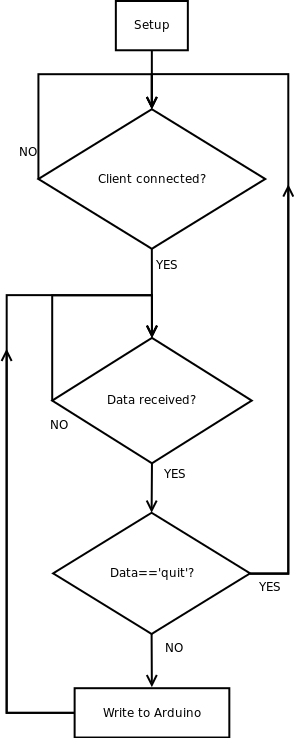
\includegraphics[scale=.8]{images/Diagrams/rasbpi.png}
      \caption{IP/UART program flowchart }
      \label{rasbpiFlowchart}
  \end{figure}
  \bigskip

	% \begin{minipage}{\linewidth}%to ensure it stays in the same page
 %  \begin{lstlisting}[label=ip-uart,caption=IP/UART Bridge, language=python  ]

 %  # Creates a socket server and dumps the received data to the Arduino

 %  from Adafruit_CharLCD import Adafruit_CharLCD
 %  from subprocess import *
 %  from time import sleep
 %  import serial
 %  import socket

 %  arduino=serial.Serial('/dev/ttyACM0', 9600)

 %  server_socket = socket.socket(socket.AF_INET, socket.SOCK_STREAM)
 %  server_socket.bind(("", 3005))
 %  server_socket.listen(1)

 %  print 'Socket started'
 %  lcd = Adafruit_CharLCD()
 %  lcd.begin(16,1)

 %  while 1:

 %    lcd.clear()
 %    lcd.message('Awaiting client')
 %    client_socket, address = server_socket.accept()
 %    lcd.clear()
 %    lcd.message('Client connected')

 %    while 1:
 %      data = client_socket.recv(4096)
 %      if data == 'quit' :
 %        break
 %      arduino.write(data)
 %      arduino.flush()

 %  \end{lstlisting}
 %  \end{minipage}







\subsection{Initializing Script} 

One of the defining features of this project is that it must be usable by non-technological people, and so it must initialize every service it needs on its own. \\

To do so, the tasks previously defined are called automatically from a script when the system boots. The contents of \textit{/etc/rc.local} are executed right after the computer executes its own routines.\\


	\begin{minipage}{\linewidth}%to ensure it stays in the same page
	\begin{lstlisting}[label=ap-default,caption=Initialization Script {[} /etc/rc.local {]} ,language=python ]
  #!/bin/bash

  #Start ip Server
  /etc/init.d/isc-dhcp-server start

  #Start webcam streaming 
  #Runs on background so this script is able to launch the next item 
  #in list
  /home/pi/mjpg-streamer/startStreaming.sh &
  sleep 0.3

  #Start Android to Arduino dumping
  /home/pi/AndroidToArduino/startA2A.sh 


  exit 0


	\end{lstlisting}
	\end{minipage}

\bigskip
The file must be given executable permissions in order to be allowed to implement the commands specified. This is done by typing \textit{sudo chmod +x /etc/rc.local} into a terminal window.